\chapter{Methods and Theoretical Background}

This chapter focuses on explaining the methods, discussing the underlying theory, and outlining key assumptions. 

\section{Exponential distribution}

Describing the distance between independent events in time, the exponential distribution is \textcolor{blue}{...} with the key property in being lack of memory. PDF is one of the defining features of a random variable $X$, and for variables coming from an exponential distribution is defined as: 

\begin{equation}
    f(x;\lambda) = \lambda e^{-\lambda x} \quad \text{for } x \ge 0 
\end{equation}

where $\lambda$ is the rate parameter. \cite{Marek2024}

\begin{figure}[h]
    \centering
    \caption{Exponential Distribution $\lambda = 1$}
    \label{fig:Exp1}
    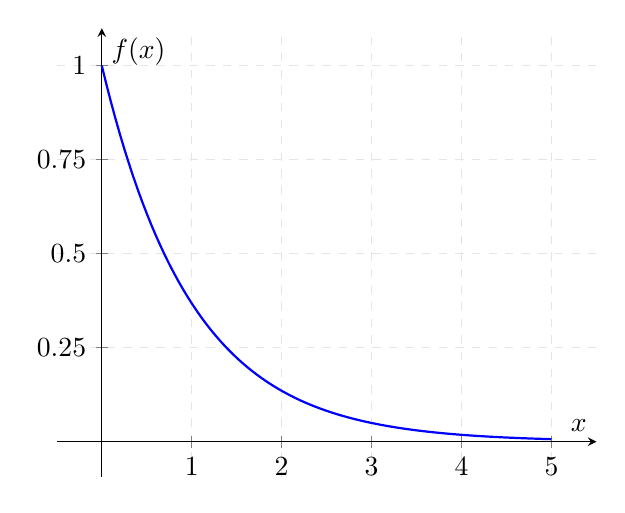
\begin{tikzpicture}
        \begin{axis}[
            domain=0:5,
            samples=100,
            axis x line=middle,
            axis y line=middle,
            xlabel={$x$},
            ylabel={$f(x)$},
            xtick={1,2,3,4,5},
            ytick={0.25, 0.5, 0.75,1},
            grid=major,
            grid style={dashed, gray!20},
            enlargelimits=true,
            %title={Exponential Distribution: $\lambda e^{-\lambda x}$ for $\lambda = 1$}
        ]
        \addplot[blue, thick] {exp(-x)};
        \end{axis}
    \end{tikzpicture}
    \source{ and processing: author}
\end{figure}

\begin{koment}
    Jak se exponencialni rozdeleni tyka BL? 

    Benfordovo rozdeleni muze pripominat exponencialni rozdeleni, proto bych mela popsat, jak to rozdeleni vypada, nakreslit nejaky pekny grafik a popsat co dela parametr lambda. Mozna by se hodil nejaky pekny priklad pouziti? 

    Mozna me jeste napada, jestli sem nenapsat co je to rozdeleni, frekventisticka definice pravdepodobnosti (since pocitam relativni frekvence vyskytu cislic na dane pozici a prirovnavam to k pravdepodobnostem) 
\end{koment}

Kdyz porovname exponencialni rozdeleni a rozdeleni podle benfordova zakona, narazime na dve vyrazne odlisnosti 
Benforduv zakon je diskretni (relativni frekvence pro jednotlive cislice), exponencialni rozdeleni je spojite. Dal, Benforduv zakon ma vetsi tails (jestli se tomu da vubec tak rikat pro diskretni rozdeleni), zatimco exponencialni rozdeleni ma tails velmi male. Pri zvoleni parametru, aby si byla rozdeleni blizka, vidime, jak jsou si odlisna. 

\begin{figure}[h]
    \centering
    \caption{Porovnani BL a Exp(0.45)}
    \label{fig:Exp0.45aBL}
    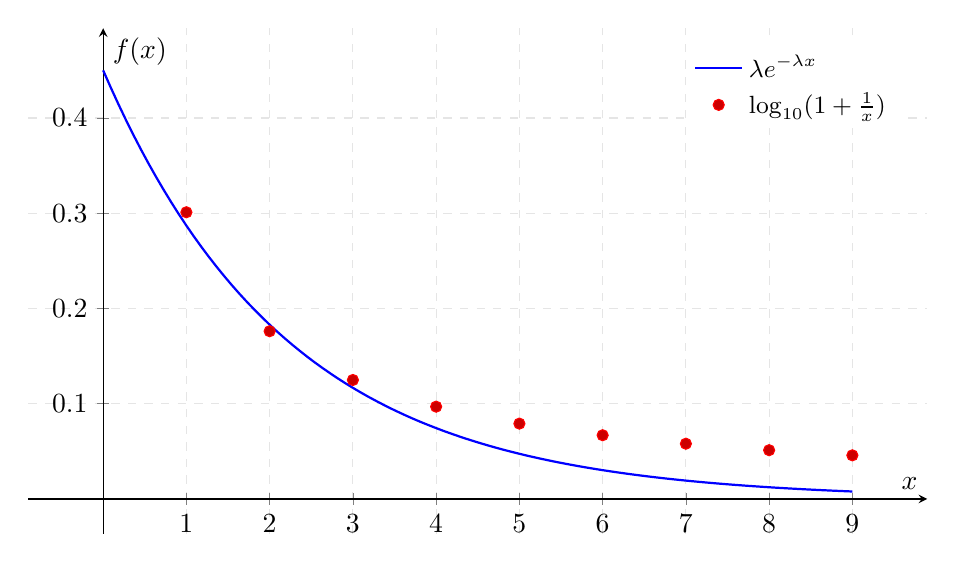
\begin{tikzpicture}
        \begin{axis}[
            width=13cm,  % Set the width of the plot
            height=8cm,  % Set the height of the plot
            domain=0:9,
            samples=100,
            axis x line=middle,
            axis y line=middle,
            xlabel={$x$},
            ylabel={$f(x)$},
            xtick={1,2,3,4,5,6,7,8,9},
            yticklabel style={/pgf/number format/.cd, fixed, precision=2}, 
            %ytick=\empty, 
            grid=major,
            grid style={dashed, gray!20},
            enlargelimits=true,
            %title={Porovnani BL a Exp(0.45)},
            legend style={draw=none, font=\small, cells={anchor=west}},
            legend pos=north east
        ]
        \addplot[blue, thick] {0.45*exp(-0.45*x)};
        \addlegendentry{$\lambda e^{-\lambda x}$}
        \addplot+[red, only marks, mark=*, mark size=2]
            coordinates {
            (1,0.3010) 
            (2,0.1761) 
            (3, 0.1249) 
            (4,0.0969) 
            (5,0.0791) 
            (6,0.0669) 
            (7,0.0580) 
            (8,0.0512) 
            (9,0.0458)
            };
        \addlegendentry{$\log_{10}(1 + \frac{1}{x})$}

        \end{axis}
    \end{tikzpicture}
    \source{ and processing: author}
\end{figure}


% %It is a non negative function, which sum equals to one. 

% For continuos variable is it defined as 

% \begin{equation}
%     P(x_1 \le X \le x_2) = \int\limits_{x_1}^{x_2} f (x) dx
% \end{equation}

% The distribution function is defined as 

% \begin{equation}
%     F(x) = P(X \le x), \quad \forall x \in R
% \end{equation}

% \begin{equation}
%     F(x) = \int\limits_{-\infty}^{x} f (t) dt, \quad -\infty <x<\infty
% \end{equation}

% \begin{koment}
%     neklesajici, v $-\infty$ je 0, v $\infty$ je 1

%     vymyslet jak to pojmout a propojit? 
% \end{koment}

\section{Hypothesis testing}

\subsection{First and second order errors (alpha beta)}

\subsection{P-value}

\subsection{Compliance to BL testing}

\subsubsection*{$\chi^2$ goodness of fit test}

To check the compliance of the data to the BL, we can use the $\chi^2$ goodness of fit test. The null hypothesis is that we assume the empirical distribution follows the theoretical BL distribution. The test criterion is given as such 

\begin{equation}
    \label{chi-sq-test}
    G= n \sum\limits_{d=1}^{9} \frac{(p_d -\pi_d)^2}{\pi_d} 
\end{equation}

\begin{align*}
    \text{where } &\pi_d \text{ is the theoretical frequency under BL distribution}, \\
    &p_d \text{ is the empirical frequency from the data, and} \\ 
    &n \text{ is the sample size}
\end{align*} 

as recommended in \citeauthor{Hronova2023}, \citeyear{Hronova2023} and  \citeauthor{kossovsky2014benford}, \citeyear{kossovsky2014benford}. %asi i Kossovsky

% \begin{koment}
%     Pozor na stanovení N při testování pomocí chisq testu.
%     Je tam důležité odlišit, co je skutečně ta reálná populace - uvádí na příkladu, že populace mohou být sales revenue za celé čtvrtletí (57 tisíc záznamů) - unique price list, unique products... ale třeba sales revenue z malého coffee shopu bude třeba k nějaké populaci přihodit - je zde možné testovat compliance a u toho velkého vzorku ne? Nevím, jestli to chápu dobře... 

%     Pokud ten dataset existuje sám o sobě in its unique fashion, je to potom comparison, ne compliance. Compliance to bude když testujeme (za použití statistického testu) nějaký náhodný výběr. (takže třeba hlasy jen pro jednoho z kandidátů?) 

%     Pak se dal ukazují Z testy (pro jednotlivá pozorování) a pak ChiSq test pro cele. Nakonec je pak jeste zajimava smerodnatna odchylka jako measure odlisnosti. 
% \end{koment}

\subsubsection*{Z test}

This test is performed individually on a particular digit/combination, however, the false positive error (type I) is more likely for the overall test of the chi-square.

Null hypothesis: Data obeys Benford's Law in the context of the particular digit/combination. % this individual observation obeys the benfords law ? 

\begin{equation}
    \label{z_test}
    Z_d = \frac{|P_o - P_e| - 1/2n}{\sqrt{(P_e(1-P_e)/n}}
\end{equation}

\begin{align*}
    \text{where } &P_o \text{ is the observed frequency of the particular digit/combination}, \\
    &P_e \text{ is the expected Benford proportion for the particular digit/combination, and} \\ 
    &n \text{ is the sample size}
\end{align*} 

We reject the null hypothesis when the $Z_d$ value is larger than $Z$ with the hladina významnosti alpha. $Z$ refers to the Standardized Normal Distribution, a Normal distribution with mean 0 and standard deviation 1. 

\subsubsection*{Kolmogorov-Smirnov test}

\section{Benford's Law Formulation}

The relative frequency of a leading digit approaches 

\begin{equation}
    \label{BZ-general_first}
\text{P(} X = d_i\text{)}= \log_{10}(1+1/d_i)
\end{equation}

where $d_i \in \{1,\dots,9\}$ for first digit law and $d_i \in \{10,\dots,99\}$ for the first-two digits law or even $d_i \in \{100,\dots,999\}$ for the first-three digits law. When plotted, it resembles nice logarithmic distribution, as seen on figure \ref{fig:FL}.  \cite{Cerqueti2202,Hronova2023,Newcomb1881}

\begin{figure}[h]
    \centering
    \caption{Theoretical frequencies of the first leading digits}
    \label{fig:FL}
    \pgfplotsset{width=8.5cm,compat=1.18}
        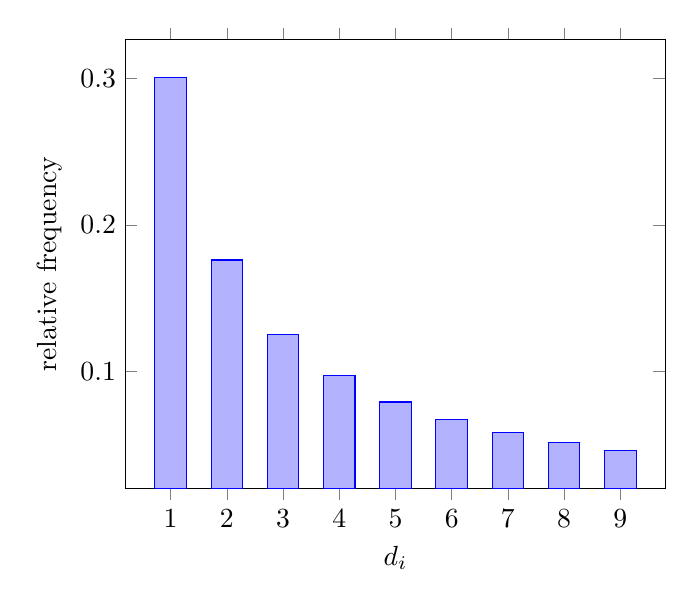
\begin{tikzpicture}
            \begin{axis}[
                ybar,
                bar width=.4cm,
                enlargelimits=0.1,
                ylabel={relative frequency},
                xlabel={$d_i$},
                symbolic x coords={1,2,3,4,5,6,7,8,9},
                xtick=data,
                ]
            \addplot coordinates {(1,0.3010) (2,0.1761) (3, 0.1249) (4,0.0969) (5,0.0791) (6,0.0669) (7,0.0580) (8,0.0512) (9,0.0458)};
            \end{axis}
        \end{tikzpicture}
    \source{ and processing: author}
\end{figure}

The first leading digit is the one found at the highest order and is non-zero. In the case of the number 124.857, the first digit would be 1, whereas for the number 0.03958, the first digit would be 3. According to Benford's law of the first digit, the theoretical frequencies correspond to the equation \ref{BZ-general_first}, indicating that the digit 1 occurs in the first position with a probability of 0.3, the digit 2 with 0.18, and so forth, with the digit 9 occurring with a probability of only 0.046.
%Compliance to this distribution is the first step in the nine-step procedure recommended by \citeauthor{kossovsky2014benford}, as mentioned in section \ref{correct_usage}.

As can be seen in the graph \ref{fig:FL}, the distribution is heavily skewed in favour of the lowest digits. As we move to the second (figure \ref{fig:second-digit-law}) and higher digits, this skew will flatten out significantly until there is no difference between the digits.  \cite{kossovsky2014benford}

This can be described by 

\begin{equation}
    \label{BZ-general_second}
    P(d) = \sum\limits_{k=1}^{9} \log_{10}\left( 1+\frac{1}{10k+d}\right), \quad \text{for } d = 0,1,\dots,9
\end{equation}

as mentioned by \citeauthor{Hronova2023} in \citeyear{Hronova2023}, assuming the independent occurence of the second leading digits. 

\begin{figure}[h]
    \centering
    \caption{Theoretical frequencies of the second leading digits}  
    \label{fig:second-digit-law}
        \pgfplotsset{width=8.5cm,compat=1.18}
            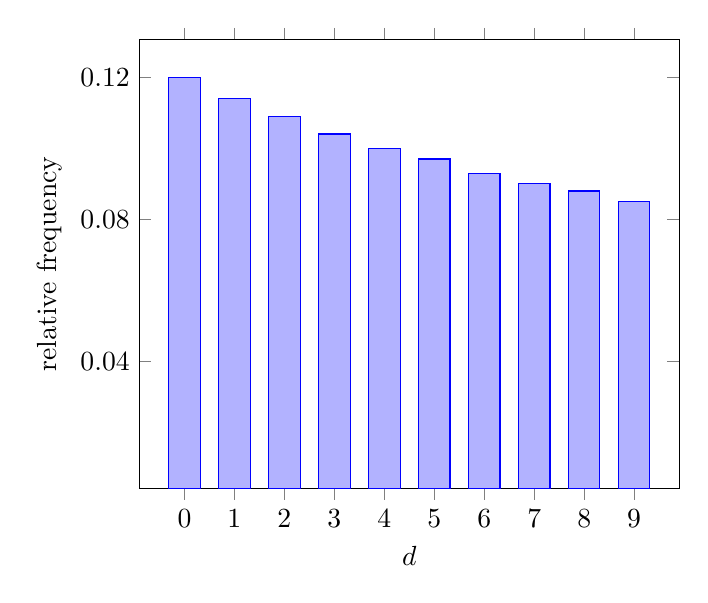
\begin{tikzpicture}
                \begin{axis}[
                    ybar,
                    bar width=.4cm,
                    ymin=0.015,
                    ytick={0.12, 0.08, 0.04},
                    enlargelimits=0.1,
                    ylabel={relative frequency},
                    xlabel={$d$},
                    symbolic x coords={0, 1,2,3,4,5,6,7,8,9},
                    xtick=data,
                    yticklabel style={/pgf/number format/fixed, /pgf/number format/precision=2},
                    ]
                \addplot coordinates {(0,0.12) (1,0.114) (2,0.109) (3, 0.104) (4,0.10) (5,0.097) (6,0.093) (7,0.09) (8,0.088) (9,0.085)};
                \end{axis}
            \end{tikzpicture}
    \source{: \citeauthor{kossovsky2014benford}, \citeyear{kossovsky2014benford}; processing: author}
\end{figure}

The distribution for the second digits is less skewed than that of the first leading digits. 
%Compliance to this distribution is the second step in the nine-step procedure recommended by \citeauthor{kossovsky2014benford}, as mentioned in section \ref{correct_usage}.
Coming to the third leading digit, the relative frequencies start to be close to equal as seen on figure \ref{fig:third-digit-law}. \cite{kossovsky2014benford}

This is explained by the following equation 

\begin{equation}
    P(d) = \sum\limits_{d_1=1}^{9} \sum\limits_{d_2=1}^{9} \dots \sum\limits_{d_{k-1}=1}^{9}   \log_{10}\left( 1+\frac{1}{\sum\limits_{i=1}^{k} d_i \cdot 10^{k-i} }\right), \quad \text{for } d_k = 0,1,\dots,9 
\end{equation}

describing third and following position relative frequencies, again with the assumption of independence of digit occurrences. And \uv{\emph{the Benford distribution converges to a uniform
multinomial distribution}} as put in \citeauthor{Hronova2023} in \citeyear{Hronova2023}. 

\begin{figure}[ht]
    \centering
    \caption{Theoretical frequencies of the third leading digits}  
    \label{fig:third-digit-law}
    \pgfplotsset{width=8.5cm,compat=1.18}
        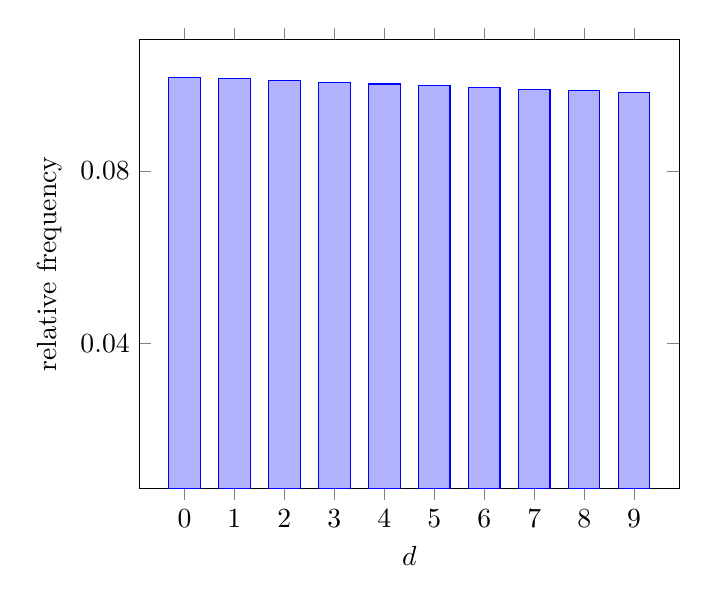
\begin{tikzpicture}
            \begin{axis}[
                ybar,
                bar width=.4cm,
                ymin=0.015,
                ytick={0.12, 0.08, 0.04},
                enlargelimits=0.1,
                ylabel={relative frequency},
                xlabel={$d$},
                symbolic x coords={0,1,2,3,4,5,6,7,8,9},
                xtick=data,
                yticklabel style={/pgf/number format/fixed, /pgf/number format/precision=2},
                ]
            \addplot coordinates {(0,0.1018) (1,0.1014) (2,0.1010) (3, 0.1006) (4,0.1002) (5,0.0998) (6,0.0994) (7,0.0990) (8,0.0986) (9,0.0983)};
            \end{axis}
        \end{tikzpicture}
    \source{: \citeauthor{kossovsky2014benford}, \citeyear{kossovsky2014benford}; processing: author}
\end{figure}

\subsection{Selected properties of numbers obeying Benford's Law}

\subsubsection{The Scale Invariance Principle of Benford's Law}

Given a dataset that already behaves according to BL, changing units (multiplying the whole dataset by the same constant) will still behave according to BL. Any arithmetic operation applied to the whole dataset does not change the underlying BL distribution. \cite{kossovsky2014benford, Hronova2023} %section 23 The Scale Invariance Principle 

\subsubsection{Digital Development Pattern}

Dividing the numbers by their orders into intervals such as (0.1,1), (1,10), (10,100) etc., we find that a pattern develops among them - the lower digits like 1 and 2 occur more frequently as the orders increase, while higher digits such as 8 and 9 gradually decrease in frequency. Data based on exponential growth should not be divided into intervals. \cite{kossovsky2014benford} % section 24

\begin{koment}
Comment on the conditions of what the dataset has to meet! 
%Aby BZ platil, musí být čísla - soubor čísel, takzvaně \emph{benfordovský} - dostatečně velký a splňovat podmínku \ref{BZ-podminka} \cite{kossovsky2014benford}. %section 10
\end{koment}

\subsection{Applicability of Benford's Law}

The law does not impose many conditions on the data that will be analysed, yet some must be met for reliable results. This section will discuss the following. 

\citeauthor{kossovsky2014benford} notes that for data to behave according to BL, its range should be wider, rather than narrow. He describes a measure \textbf{Order of Magnitude of Variability (OMV)} as:  

\begin{equation}
    OMV = \log(\text{90th percentile}) - \log(\text{10th percentile}) > 3 
    \label{OMV}
\end{equation}

and recommends it should be larger than 3. In practice, this means that our data should spread all the way from 1 to 10000 or more for consistent results. 
 
\subsubsection*{Correct usage} 

The compliance of our data with the law can be expected when only minimal conditions are met. Then the conformity can be tested. This makes the law good for detecting the presence of fraud or various manual manipulations of numbers with high accuracy. \cite{kossovsky2014benford, Cerqueti2202,kossovsky2014benford} 

When using Benford's Law to detect intentional fraud or data manipulation, the complete dataset is used, rather than a subset. Additionally, the dataset must satisfy conditions other than those mentioned in the previous chapters. The dataset should be large enough - for datasets with less than 100 observations, BL analysis is not recommended. %\cite{kossovsky2014benford} % section 26, strana 82
Only non-negative data should be used for analysis. For use in auditing, it is also recommended to eliminate small numbers, values less than, for example, 50, but that the portion removed be less than $10\%$. In addition, values that represent totals, summations, etc., should not be included if they come from the same sample. \cite{kossovsky2014benford} % section 27, strana 88 

\subsubsection*{Varying results from the expected distribution}

It is generally advisable to focus on deviations from the theoretical distribution in a given BL variation, specifically on the significantly higher values for the frequency of occurrence of a given digit. In graphical representation, these can be represented as spikes. There is minimal interest in the reduced frequencies, as any suspicious activity is likely to manifest itself through increased frequencies - when counting frequencies, an increase in one digit is much more detectable, with all other frequencies dropping slightly. \cite{kossovsky2014benford} % section 26, strana 85 

% \begin{koment}
%     grafický příklad jak vypadá hrot jakožto odchylka od konformity s BZ - pokud nebudu mít nic svého, Kossovsky strana 83. Potom i další ukázky podivných situací.
% \end{koment}

%There will always be variation, because few datasets are $100\%$ \textit{Benfordian}.  \cite{kossovsky2014benford} % section 26, strana 84

Deviance is to be expected, but where should the line be drawn?  \citeauthor{kossovsky2014benford} suggests distinguishing between two terms: compliance and comparison. When researching the data's compliance with BL, the data is expected to follow the logarithmic distribution very closely, the focus is on detecting manipulation, and if there is, whether it is random or structural. For comparison, the conditions are much looser. We don't assume any \textbf{prior population type (logarithmic distribution)}. For our use, we will be assuming the data should follow the distribution and therefore observe data compliance.


Next, the deviations should not show signs of any systematic error or pattern. Some pattern may emerge by rounding numbers, for example. The practice of rounding data is prevalent in the context of accounting, where values ending in 00 or 50 are frequently observed. This rounding process, which is often employed to streamline computations, can give rise to manipulation of higher orders while being harmless in context. Empirical evidence supports the prevalence of these values in practice. %\cite{kossovsky2014benford} %section 27, strana 92
However, such manipulations are unacceptable in, for example, electoral statistics, where votes simply cannot be rounded.
\cite{kossovsky2014benford}

% \begin{koment}
%     * insert příklad z analýzy volebních výsledků v Rusku, kde se zaokrouhlovalo, nebo odkaz na vyssi kapitolu kde se k tomu snad dostanu * 
% \end{koment}

There are also numbers that someone must have made up at some point. In accounting, donations are a good example. That is a number that someone has determined. Just as, for example, prizes. Such numbers do not follow BL and will show high degrees of deviation. \cite{kossovsky2014benford}

Alternatively, the validity of BL can be influenced by changed external situations in regards to the data itself. For instance, how does sales data follow BL distribution when affected by the pandemic in 2020? This has been answered by \citeauthor{Hronova2023} in \citeyear{Hronova2023}. Changes like this should be taken into account, and analysis should be adapted accordingly.


\subsection{Forensic digital analysis tests}

When detecting similar errors, it is often not enough to only look at the first digits' distribution. It is advised to look at the last two digits to detect rounding. For a comprehensive analysis, \citeauthor{kossovsky2014benford} recommends following tests:

\begin{enumerate}
    \item First-digits distribution
    \item Second-digits distribution
    \item Combination of the first-two-digits distributions
    \item Combination of the first-three-digits distributions
    \item Combination of the last-two-digits distributions 
    \item Examination of first-order digital development
    \item Examination of second-order digital development
    \item Value repetition test
    \item Observing the Digital Development and BL Pattern among it 
    \item Summation test   
\end{enumerate}

These tests, as they are generally very important to include, do not make any sense in our analysed data. Value repetition test is advised to be useful for data from the accounting or financial sector, digital development is not interesting since the election districts are set to be a particular size and summation test is not making any sense to be used in election analysis. 

% \subsubsection*{Combination of distributions}

\begin{koment}
    Popravdě, mám chuť toto skipnout, Summation test mi nedává v kontextu voleb až takový smysl, myslím, že ho vynechám. Value repetition test je doporučen pro accounting a financial data. Digital development je essential, na ten se musím podívat.  

    Jenže u toho je problém v tom, že volební okrsky jsou fixed na 1000 obyvatel, tudíž ten development nebude moc velkej. Co okresní data? Mám pocit, že se to mé práce taky úplně netýká. 
\end{koment}


\subsubsection*{Examination of a digital development}

Digital development pattern refers to the way distributions of digits evolve across different ranges of data. This pattern is observed in all random data sets, whether they follow Benford's Law or not. The pattern shows how the distribution of digits changes from lower to higher values of the data range. 

This pattern can only be seen when the data range is partitioned along integral powers of ten, such as (0.1, 1), (1, 10), (10, 100), etc. The pattern shows increasing skewness as you move from the left to the right of the data range. For smaller values, digit distributions are more equal. In the centre, the distribution becomes more logarithmic. For larger values, the distribution becomes highly skewed in favour of low digits. \cite{kossovsky2014benford}


% \subsubsection*{Value repetition test}

% \subsubsection*{Summation test}




\section{Analysis workflow}

This is the proposed analysis workflow for this thesis: 


Preprocessing: 

\begin{enumerate}
    \item load data 
    \item clean data - remove summations and totals 
    \item extract digits for analysis into separate datasets (first, last, first two, last two) 
\end{enumerate}

Analysis itself: 

\begin{enumerate}
    \item[4.] Is data fit for applying BL? (velikost okrsku, min max vzdalenost a tak)
    \item[5.] First leading digits compliance to BL
    \item[6.] Last digits test (their relative frequency is from the Uniform distribution)
    \item[7.] Summation test 
    \item[8.] Value Repetition test
\end{enumerate}
